\documentclass[12pt]{article}

\usepackage[T1]{fontenc}
\usepackage[utf8]{inputenc} % L'encodage du document
\usepackage[french]{babel} % Des options supplémentaires pour que le document soit en français (noms de sections, etc.)
\usepackage{geometry}
\geometry{hscale=0.80,vscale=0.80,centering} % Permet de définir les marges (ici 10% de chaque côté)
\usepackage{amsmath}
\usepackage{amssymb}
\usepackage{amsthm} % For theorem-like environments
\usepackage{graphicx} % Ajout du package graphicx
\usepackage{minted}
\usepackage{fixltx2e}
\usepackage{array}
\usepackage{lettrine}
\usepackage{tikz}
\usetikzlibrary{angles,quotes}

\newcolumntype{C}[1]{>{\centering\arraybackslash}m{#1}}
\newcolumntype{L}[1]{>{\raggedright\arraybackslash}m{#1}}
\newcolumntype{N}{@{}m{0pt}@{}}

\newcounter{definitioncounter}
\renewcommand{\thedefinitioncounter}{\arabic{definitioncounter}}

\newcommand{\definition}[1]{%
    \par\noindent\textbf{Définition \refstepcounter{definitioncounter}\thedefinitioncounter.} #1 \vspace{0.5\baselineskip}
}

\newcommand{\fig}[1]{
    F\resizebox{!}{1.3ex}{IGURE} #1
}

\newcounter{propositioncounter}
\renewcommand{\thepropositioncounter}{\arabic{propositioncounter}}

\newcommand{\proposition}[1]{%
    \par\noindent\textbf{Proposition \refstepcounter{propositioncounter}\thepropositioncounter.} #1 \vspace{0.5\baselineskip}
}

\setlength{\parindent}{15pt} % Fixe l'indentation en début de paragraphe
\setlength{\parskip}{10pt} % Fixe l'espacement entre paragraphes

\begin{document}
\title{Simuler les feux de forêt}
\date{\today}
\author{Victor Sarrazin}

\maketitle

\section*{Introduction}

Avec le changement climatique, les feux de forêt sont de plus en plus fréquents et dévastateurs, à l'image de ceux en Californie en janvier 2025.

Dans ce cadre, les modélisations informatiques des feux de forêt permettent de simuler leur évolution et ainsi de prévoir les zones à risque. Elles offrent également la possibilité de tester l'impact de certaines transformations sur ces incendies, afin d'identifier des moyens de réduire les conséquences des catastrophes sans dénaturer les forêts.

\section{Automates cellulaires}

\subsection{Généralités}

Pour réaliser nos modélisations, nous allons utiliser des automates cellulaires. Ces outils permettent de représenter des systèmes avec des interactions locales entre les éléments qui les constituent. Les automates cellulaires ont notamment été popularisés avec \textit{Le~Jeu~de~la~Vie} de \textit{Conway}.

\definition{Un automate cellulaire est la donnée d'un triplet $(Q, M, f)$ avec :\begin{itemize}
    \item $Q$ un ensemble d'états
    \item $M$ une matrice de taille $n \times m$, où chaque $m_{i,j}$ représente une cellule de la grille
    \item $f : \mathcal{M}_{n,m}(Q) \longrightarrow \mathcal{M}_{n,m}(Q)$ une \textit{fonction de transition} qui à une grille renvoie la grille suivante
\end{itemize}}

La définition de la fonction de transition dépend donc du type de voisinage considéré. Il existe deux principaux types de voisinages : celui de \textit{von Neumann} et celui de \textit{Moore}. Nous avons choisi d'utiliser le voisinage de \textit{Moore} pour nos modélisations pour prendre en compte le plus d'intéractions possibles, celui de \textit{von Neumann} étant plus limitatif, notamment en ce qui concerne les interactions diagonales.

\definition{Le voisinage de \textit{Moore} est composé de la cellule centrale et de ses 8 voisins adjacents (horizontalement, verticalement et diagonalement).}

\begin{figure}[!ht]
    \centering
    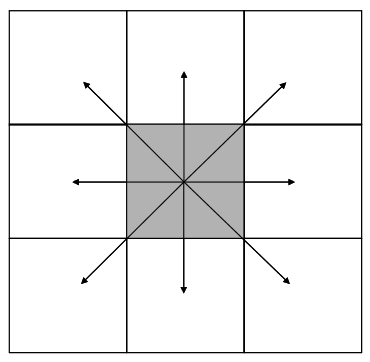
\includegraphics[width=0.20\linewidth]{pictures/moore.png}
    \caption{Voisinage de Moore}
    \label{fig:enter-label}
\end{figure}

Il serait possible dans une optique d'avoir des modèles encore plus précis d'utiliser des voisinages de \textit{Moore} étendus, avec plusieurs rayons de voisins. Cependant par souci de simplicité nous nous sommes restreints à un rayon.

\subsection{Représentation d'un forêt}

Afin de représenter une forêt avec un automate cellulaire, nous avons défini une liste d'états que les cellules pouvaient prendre.

\definition{Les états possibles sont :
\begin{itemize}
    \item Arbres
    \item Arbres denses
    \item Champs
    \item Feu
    \item Case brûlée\textsuperscript{*}
    \item Eau\textsuperscript{*}
\end{itemize}
A noter que les cases $(*)$ ne peuvent brûler.}

Nous avons choisi de travailler avec une matrice de taille $256 \times 256$ pour des raisons techniques : au-delà le temps de calcul devenait trop long, et l'ajout de lignes/colonnes ne représentait pas un intérêt suffisant au regard du temps de calcul que cela impliquait.

\section{Modèle d'Alexandridis}

Dans un premier temps, il est possible de réaliser une modélisation simple des feux de forêt en associant à chaque cellule une probabilité fixe de s'enflammer si l'un de ses voisins est en feu. Une telle tentative a donné des résultats mitigés. C'est pourquoi l'objectif de cette deuxième partie est de présenter un modèle plus avancé de modélisation des feux de forêts, appelé modèle d'\textit{Alexandridis}.

\subsection{Présentation du modèle}

Le modèle d'\textit{Alexandridis} prend en compte divers phénomènes pour simuler la propagation des incendies. Par la suite, nous avons choisi de nous concentrer sur la densité de végétation, le type de végétation ainsi que le vent dans la zone. Le modèle original prend également en considération l'élévation du terrain.

\proposition{On utilise les règles de transition suivantes, pour $(i,j) \in \mathbb{N}^2$, $t \in \mathbb{N}$ :
\begin{itemize}
    \item Si $m_{i,j} (t) = $ \mintinline{latex}{feu} alors $m_{i,j} (t+1) = $ \mintinline{latex}{brulé}
    \item Si $m_{i,j} (t) = $ \mintinline{latex}{feu} alors $m_{i \pm 1,j \pm 1} (t+1) = $ \mintinline{latex}{feu} avec une probabilité $p_b$
    \item Si $m_{i,j} (t) = $ \mintinline{latex}{brulé} alors $m_{i,j} (t+1) = $ \mintinline{latex}{brulé}
\end{itemize}}

\proposition{La probabilité $p_b$ qu'une cellule brûle est définie par
$p_b = p_h (1 + p_{veg}) (1 + p_{den}) p_{vent}$ avec $p_h = 0.27$ une constante, et $p_{veg}$ et $p_{den}$ des coefficients relatifs au type de cellule.
}

\begin{figure}[!ht]
    \centering
    \renewcommand{\arraystretch}{2}
    \setlength{\extrarowheight}{-3pt}
    \begin{tabular}{ |>{\centering\arraybackslash}p{4cm}|>{\centering\arraybackslash}p{2cm}|>{\centering\arraybackslash}p{2cm}| }
        \cline{2-3}
        \multicolumn{1}{c|}{} & $p_{veg}$ & $p_{den}$ \\
        \hline 
        Arbres & $0.3$ & $0.3$ \\ 
        \hline
        Arbres denses & $0.3$ & $0$ \\ 
        \hline
        Champs & $-0.1$ & $0$ \\
        \hline 
    \end{tabular}
    \caption{Probabilités $p_{veg}$ et $p_{den}$ selon le type de végétation}
\end{figure}

\proposition{La probabilité $p_{vent}$ liée au vent est définie par
\\ $p_{vent} = \exp (0.045 v) \times \exp (0.131 v \times (\cos (\theta) - 1))$ avec $\theta$ l'angle entre la propagation du feu et la direction du vent, et $v$ la vitesse du vent (en $m/s$)
}

\begin{figure}[!ht]
    \centering
    \begin{tikzpicture}[> = stealth]
        \coordinate (a) at (1,4);
        \coordinate (b) at (2,5);
        \coordinate (c) at (5,4);
        \coordinate (d) at (6,4);
        \coordinate (e) at (9,5);
        \coordinate (f) at (10,4);
        
        \draw pic[draw,fill=green!30,angle radius=1cm,"$\theta_1$" shift={(6mm,1mm)}] {angle=c--a--b};
        \draw pic[draw,fill=green!30,angle radius=2cm,"$\theta_2$" shift={(6mm,1mm)}] {angle=f--d--e};
        
        \draw[ultra thick,red, ->]  (a) -- node[above left] {\normalsize Vent} (b);
        \draw[ultra thick,blue,->]  (a) -- node[below] {\normalsize Propagation du feu} (c);

        \draw[ultra thick,red, ->]  (d) -- node[above left] {\normalsize Vent} (e);
        \draw[ultra thick,blue,->]  (d) -- node[below] {\normalsize Propagation du feu} (f);
    \end{tikzpicture}
    \caption{Configurations de vent}
\end{figure}

On a $\theta_1 > \theta_2$ et une vitesse plus élevée dans la seconde situation, ainsi la probabilité $p_{vent}$ sera plus élevée dans la seconde situation.

\subsection{Résultats}

Comparons d'abord les résultats de la modélisation naïve avec ceux du modèle d'\textit{Alexandridis} :

\begin{figure}[!ht]
    \centering
    \begin{minipage}{0.35\textwidth}
      \centering
      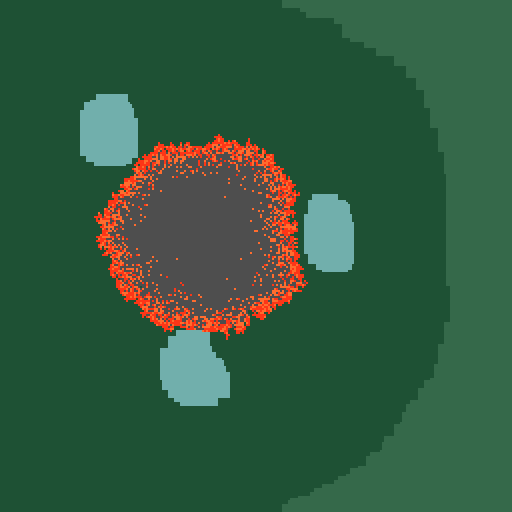
\includegraphics[width=.8\linewidth]{pictures/model1/land_200.png}
      \caption{Solution naïve}\label{Fig:Data1}
    \end{minipage}
    \hfil
    \begin{minipage}{0.35\textwidth}
      \centering
      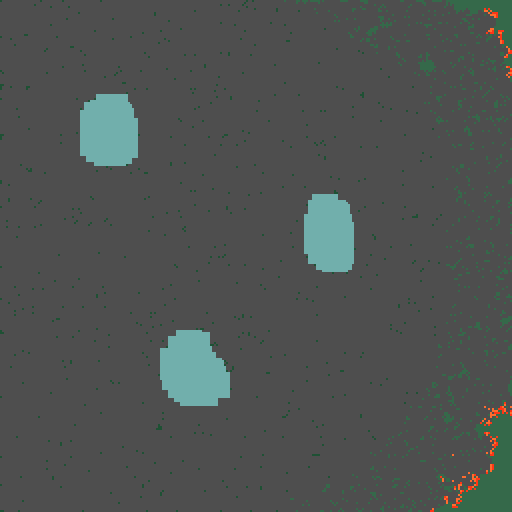
\includegraphics[width=.8\linewidth]{pictures/model2/land_200_nowind.png}
      \caption{\textit{Alexandridis}}\label{Fig:Data2}
    \end{minipage}
 \end{figure}

On observe que la solution naïve présente une propagation plus lente et un front de feu plus étendu que le modèle d'\textit{Alexandridis}.

Comparons maintenant deux modélisations du modèle d'Alexandridis avec des densités de végétation différentes, sous un vent de $15 m/s$ orienté vers l'est :

\begin{figure}[!ht]
    \centering
    \begin{minipage}{0.35\textwidth}
      \centering
      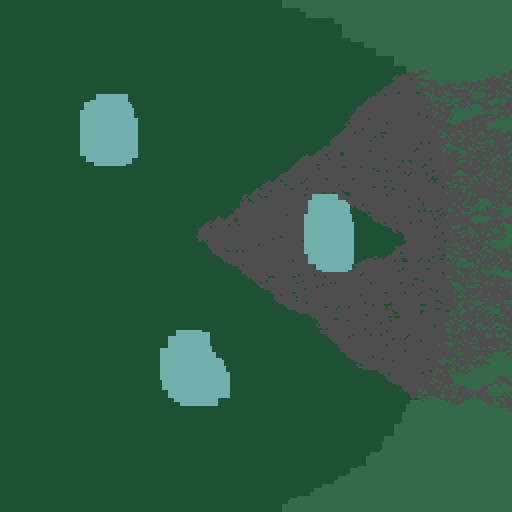
\includegraphics[width=.8\linewidth]{pictures/model2/land_200_wind_notdense.png}
      \caption{Végétation normale}\label{Fig:Data3}
    \end{minipage}\hfil
    \begin{minipage}{0.35\textwidth}
      \centering
      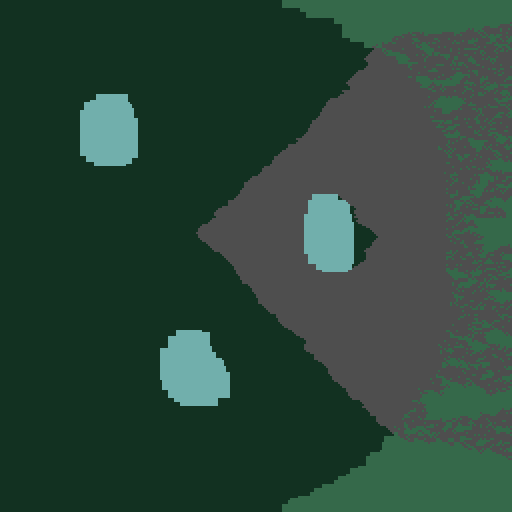
\includegraphics[width=.8\linewidth]{pictures/model2/land_200_wind_dense.png}
      \caption{Végétation dense}\label{Fig:Data4}
    \end{minipage}
 \end{figure}

On remarque principalement deux effets importants sur les deux modélisations.

Premièrement, la progression du feu dans une végétation normale est plus lente (ce qui est cohérent avec l'observation empirique), et le front de feu est donc moins étendu. La surface brûlée dans le cas de la densité normale présente également des zones non brûlées, contrairement à celle de la densité élevée qui est plus uniforme. Ce phénomène s'explique par une probabilité $p_b$ plus élevée pour une densité plus forte.

Deuxièmement, dans les deux modélisations, l'impact du vent est clairement visible : le front de feu s'est propagé selon un cône poussé par le vent.

\subsection{Considérations algorithmiques}

Cette sous-partie a pour objectif de présenter l'implémentation de la modélisation réalisée et de justifier le choix d'une grille de taille $256 \times 256$.

Voici les complexités temporelles des différentes fonctions créées :

\begin{itemize}
    \item Calcul de $p_b$ : $O(1)$
    \item Calcul du passage de l'état à l'instant $t$ à l'état à l'instant $t+1$ : $O(n^2)$, où $n$ est la dimension de la grille. Cette estimation repose sur environ $100$ opérations élémentaires (lectures, comparaisons, affectations, calculs arithmétiques, etc.) pour chaque cellule.
    \item Affichage de l'état à l'instant $t$ : $O(m^2 \times n^2)$, où $n$ est la dimension de la grille et $m$ est la taille en pixels d'une cellule représentée à l'écran.
\end{itemize}

Ainsi, pour $N$ itérations, la complexité totale est de $O(m^2 \times n^2 \times N)$. Numériquement, avec $n$ = 256, $m$ = 2 et $N$ = 200 on trouve $\approx 10^5$, et donc on en déduit grossièrement $\approx 10^7$ opérations élémentaires.

En considérant un temps d'exécution moyen par opération élémentaire, cela correspond grossièrement à un temps de calcul d'environ 5 secondes.

On comprend donc pourquoi augmenter la valeur de $n$ (toutes choses égales par ailleurs) ou de $N$ conduirait à des simulations plus longues.

\section{Transformations}

Puisque nous disposons maintenant d'un modèle pour réaliser des simulations, nous allons nous intéresser aux transformations réalisables, notamment ici, dans le cadre de cette étude, aux tranchées et chemins.

\subsection{Explications}

Nous allons donc considérer l'ajout de tranchées ou de chemins forestiers, des transformations légères qui permettent de limiter l'impact des feux sans dénaturer les forêts.

\proposition{On ajoute un nouvel état Chemins/Tranchées avec $p_{veg} = -0.55$ et $p_{den} = 0$ à notre modèle.}

\subsection{Résultats}

L'objectif est maintenant d'observer l'impact des tranchées avec différentes configurations de vent et de largeur de tranchées.

\subsubsection{Tranchées/Sans tranchées}

La première comparaison intéressante est d'étudier la différence de propagation du feu avec et sans tranchées.

\begin{figure}[!ht]
    \centering
    \begin{minipage}{0.35\textwidth}
      \centering
      
\includegraphics[width=.8\linewidth]{pictures/trans/no_treach.png}
      \caption{Sans tranchées}\label{Fig:Data5}
    \end{minipage}
    \hfil
    \begin{minipage}{0.35\textwidth}
      \centering
      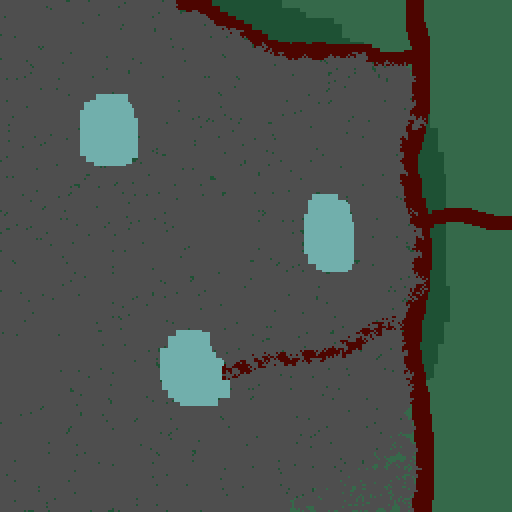
\includegraphics[width=.8\linewidth]{pictures/trans/treach.png}
      \caption{Avec tranchées}\label{Fig:Data6}
    \end{minipage}
\end{figure}

En comparant la\fig{8}et la\fig{9}on constate que la présence de tranchées permet de bloquer la propagation du feu. Il est important de noter que ce résultat est observé pour un nombre d'itérations limité (ici $200$), et qu'une simulation plus longue pourrait montrer une propagation au-delà des tranchées.

\subsubsection{Vent faible/Vent fort}

Dans un deuxième temps, comparons deux situations avec un vent orienté dans la même direction mais de vitesse différente.

\begin{figure}[!ht]
    \centering
    \begin{minipage}{0.35\textwidth}
      \centering
      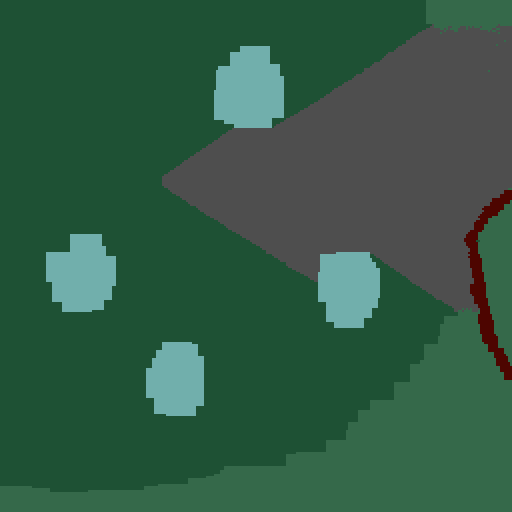
\includegraphics[width=.8\linewidth]{pictures/trans/treach_15.png}
      \caption{$15$ m/s de vent}\label{Fig:Data7}
    \end{minipage}\hfil
    \begin{minipage}{0.35\textwidth}
      \centering
      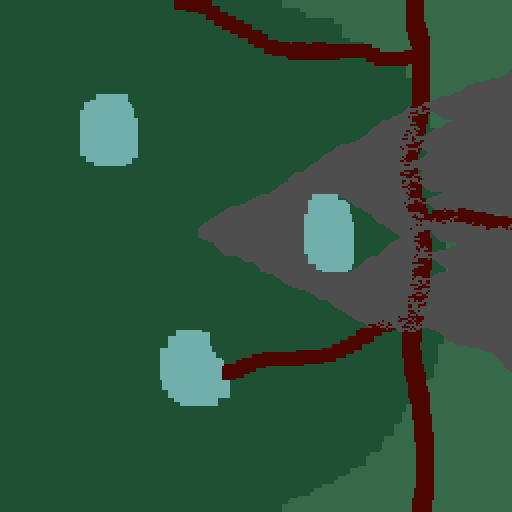
\includegraphics[width=.8\linewidth]{pictures/trans/treach_30.png}
      \caption{$30$ m/s de vent}\label{Fig:Data8}
    \end{minipage}
\end{figure}

En comparant la\fig{10}et la\fig{11}on observe qu'un vent plus fort diminue l'efficacité des tranchées ou chemins. Ce résultat est empiriquement logique : un vent plus intense permet au feu de se propager plus rapidement et donc de franchir plus facilement l'obstacle.

Il est tout de même intéressant de mentionner que, même lorsque le feu parvient à traverser la tranchée, moins de 25\% de sa surface (dans la zone impactée par le feu) est brûlée à la fin de la simulation.

\subsubsection{Tranchée mince/Tranchée large}

Dans un dernier temps, comparons deux largeurs de tranchée.

\begin{figure}[!ht]
    \centering
    \begin{minipage}{0.35\textwidth}
      \centering
      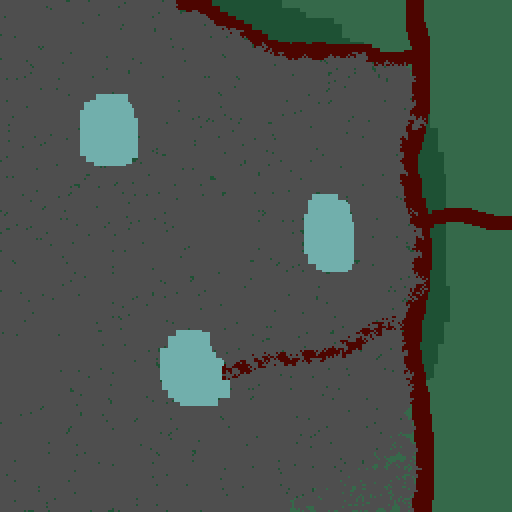
\includegraphics[width=.8\linewidth]{pictures/trans/treach.png}
      \caption{Tranchée de $8$m}\label{Fig:Data9}
    \end{minipage}\hfil
    \begin{minipage}{0.35\textwidth}
      \centering
      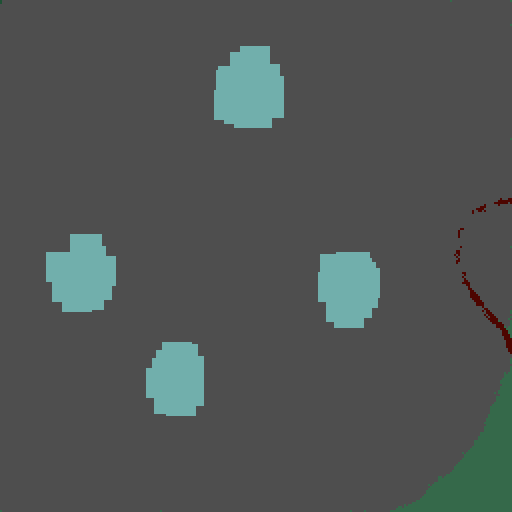
\includegraphics[width=.8\linewidth]{pictures/trans/little_treach.png}
      \caption{Tranchée de $4$m}\label{Fig:Data10}
    \end{minipage}
\end{figure}

En comparant la\fig{12}et la\fig{13}on constate qu'une tranchée plus large est plus efficace pour limiter la propagation du feu. Entre ces deux simulations, la grande tranchée verticale a été réduite horizontalement, et l'impact de ce changement est clairement visible.

De plus, on observe sur la\fig{13}que le front de feu est toujours présent, ce qui suggère qu'une simulation plus longue entraînerait la combustion d'une zone encore plus étendue.

\subsection{Possibles améliorations}

Bien que nous ayons obtenu des résultats intéressants avec ce modèle intermédiaire, qui prend en compte le type et la densité de la végétation ainsi que le vent, il est possible d'aller plus loin dans les simulations.

Il serait donc envisageable d'intégrer d'autres paramètres importants tels que l'élévation, l'humidité ou la température.

De plus, on pourrait considérer d'autres transformations pour la gestion des incendies. Par exemple, la réduction de la densité de végétation, dont la\fig{7}a permis d'observer l'impact positif sur la limitation de la propagation. Il serait également pertinent d'affiner la modélisation de l'interaction avec les cours d'eau et les lacs, qui sont actuellement considérés comme des obstacles infranchissables, alors qu'ils peuvent influencer la progression du feu de manière plus complexe.

\section{Annexe}

\subsection{Choix d'implémentation}

Pour implémenter les différents modèles, nous avons choisi le langage \mintinline{latex}{C99}. Ce choix a été principalement motivé par deux aspects :

\begin{itemize}
    \item Le bas niveau du \mintinline{latex}{C} offre un gain significatif en temps d'exécution par rapport à d'autres langages. Ceci est particulièrement avantageux compte tenu du volume important de calculs nécessaires pour simuler l'évolution des états dans nos grilles.
    \item Le \mintinline{latex}{C}, étant plus largement répandu que l'\mintinline{latex}{OCaml}, bénéficie d'un écosystème de bibliothèques externes plus vaste et plus mature.
\end{itemize}

Nous avons utilisé les bibliothèques non standard suivantes :

\begin{itemize}
    \item \mintinline{latex}{SDL2} : Pour la création d'une interface graphique permettant de visualiser l'évolution des simulations en temps réel.
    \item \mintinline{latex}{cJSON} : Pour la manipulation de fichiers \mintinline{latex}{JSON}, format utilisé pour représenter et importer les configurations initiales des grilles.
    \item \mintinline{latex}{png} : Pour la création et la manipulation de fichiers \mintinline{latex}{PNG}, afin d'exporter les résultats des simulations sous forme d'images.
\end{itemize}

Afin de faciliter la création et la configuration des grilles initiales, nous avons développé un site web interactif en \mintinline{latex}|React.JS|. Cette interface web permet de concevoir visuellement les forêts initiales avant de les exporter au format \mintinline{latex}{JSON} pour être utilisées par notre simulateur en \mintinline{latex}{C}.

\end{document}